% Appendix A

\chapter{Documentation} % Main appendix title

\label{AppendixA} % For referencing this appendix elsewhere, use \ref{AppendixA}

\lhead{Appendix A. \emph{Documentation}} % This is for the header on each page - perhaps a shortened title

%Write your Appendix content here.


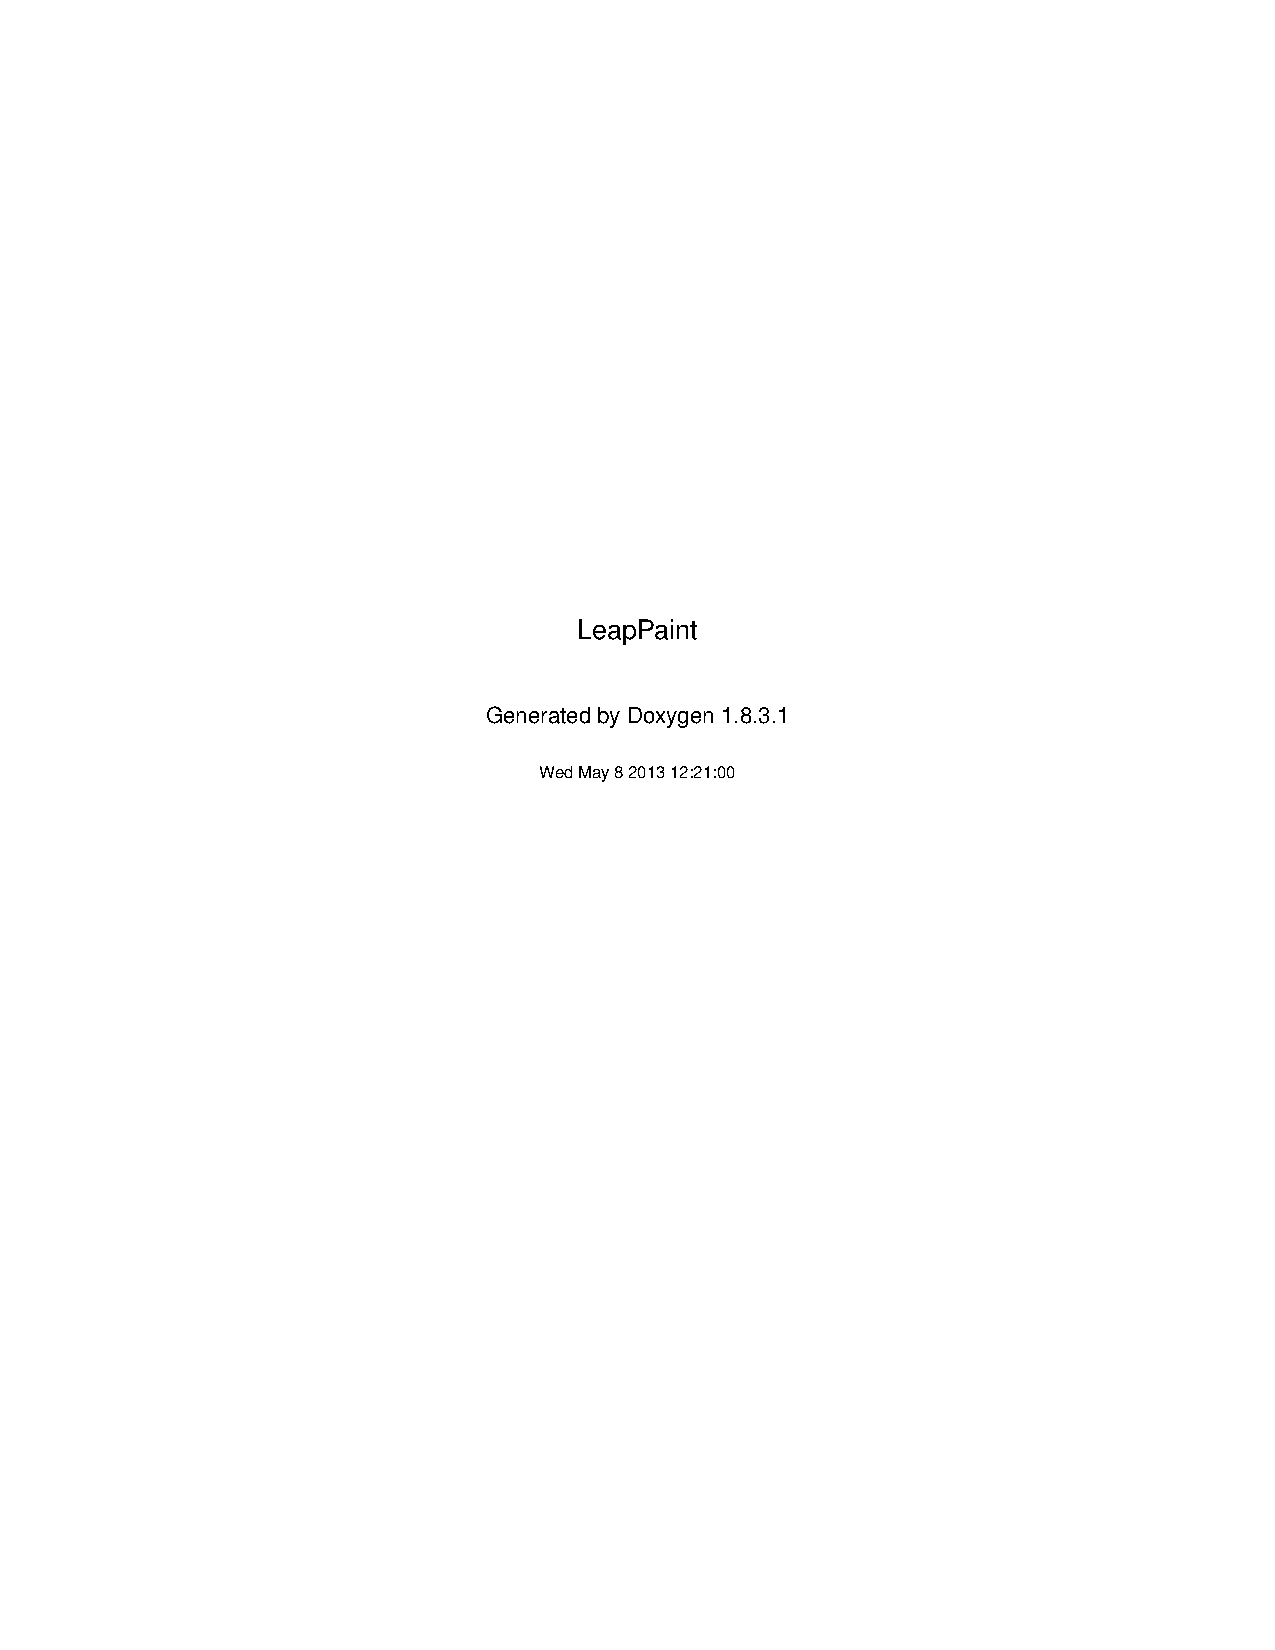
\includepdf[pages=2-last,
	    pagecommand={\thispagestyle{empty}},
            width=\textwidth+ \marginparwidth +\marginparwidth,
            height=\textheight , 
	    noautoscale,   
	    fitpaper=true,
            %offset=0pt 0pt,     %letter, oneside    => misaligned by .x pt
            offset=70pt -70pt,  %letter, twoside    => misaligned by .x pt
            %offset=0pt 0pt,    %a4paper, oneside   => misaligned by 1.x pt
            %offset=-25pt 0pt,  %a4paper, twoside   => misaligned by 1.x pt
            ]{/Users/cj/Desktop/MastersProject/LeapPaint/docs/latex/refman.pdf}


\includepdf[pages=-,
	    pagecommand={\thispagestyle{empty}},
            width=\textwidth,
            height=\textheight, 
	    noautoscale,   
	    fitpaper=true,
            %offset=0pt 0pt,     %letter, oneside    => misaligned by .x pt
           % offset=70pt 0pt,  %letter, twoside    => misaligned by .x pt
            %offset=0pt 0pt,    %a4paper, oneside   => misaligned by 1.x pt
            %offset=-25pt 0pt,  %a4paper, twoside   => misaligned by 1.x pt
            ]{/Users/cj/Desktop/MastersProject/LeapPaint/LeapPaint/code.pdf}